\documentclass[12pt,a4paper]{article}
\usepackage{amsmath}
\usepackage[T1]{fontenc}
\usepackage[utf8]{inputenc}
\usepackage{setspace}
\onehalfspacing
\usepackage{graphicx}
\usepackage{subcaption}
\usepackage{pst-tree}
\usepackage{tikz}
\usetikzlibrary{trees}
\usepackage{amsfonts}
\usepackage{amsthm}
\usepackage[top=2.5cm, bottom=2.5cm, left=2.5cm, right=2.5cm]{geometry}
\usepackage{enumerate} 
\usepackage{amssymb}
\usepackage{csquotes}
\usepackage{fancyhdr}
\usepackage{times}
\usepackage{fancyhdr}
\usepackage[bottom]{footmisc}
\pagestyle{fancy}
\usepackage{amsmath}
\usepackage{amssymb}
\usepackage{graphicx}
\usepackage{tikz}
\usepackage{lscape}
\newcommand*\circled[1]{\tikz[baseline=(char.base)]{
\node[shape=circle,draw,inner sep=2pt] (char) {#1};}}
\DeclareMathSizes{12}{12}{10}{10}
\interfootnotelinepenalty=10000
\usepackage{dsfont}
\usepackage{mathtools}
\usepackage{graphics}
\usepackage{graphicx}
\usepackage{multirow, booktabs}
\usepackage[final]{pdfpages}
\usepackage{hyperref}
\usepackage{xcolor}
\usepackage{booktabs,siunitx}
\usepackage{float}
\lhead{}
\rhead{}
\chead{}

\begin{document}
\includepdf[pages=-]{forside.pdf}
\newpage
\onehalfspacing

\tableofcontents
\newpage
\section{Introduction}
This report depicts a research performed regarding active Danish real-estate property valuations from 2016-2019. Since 2011, the yearly number of real estate properties sold has slightly increased, with 2017 being the year with most sold properties in 10 years (Danmarks Statistik, 2018).  The price of real estate properties is also rising through 2019 (Danmarks Statistik, 2019). Although this generally depicts a willingness of buyers to pay more for real-estate property, and higher valuations from agents, a closer analysis of current and active valuations contributes with local view of which conditions contribute to the valuation of a real-estate property. \newline
\begin{figure}[H]
\centering
\caption{}
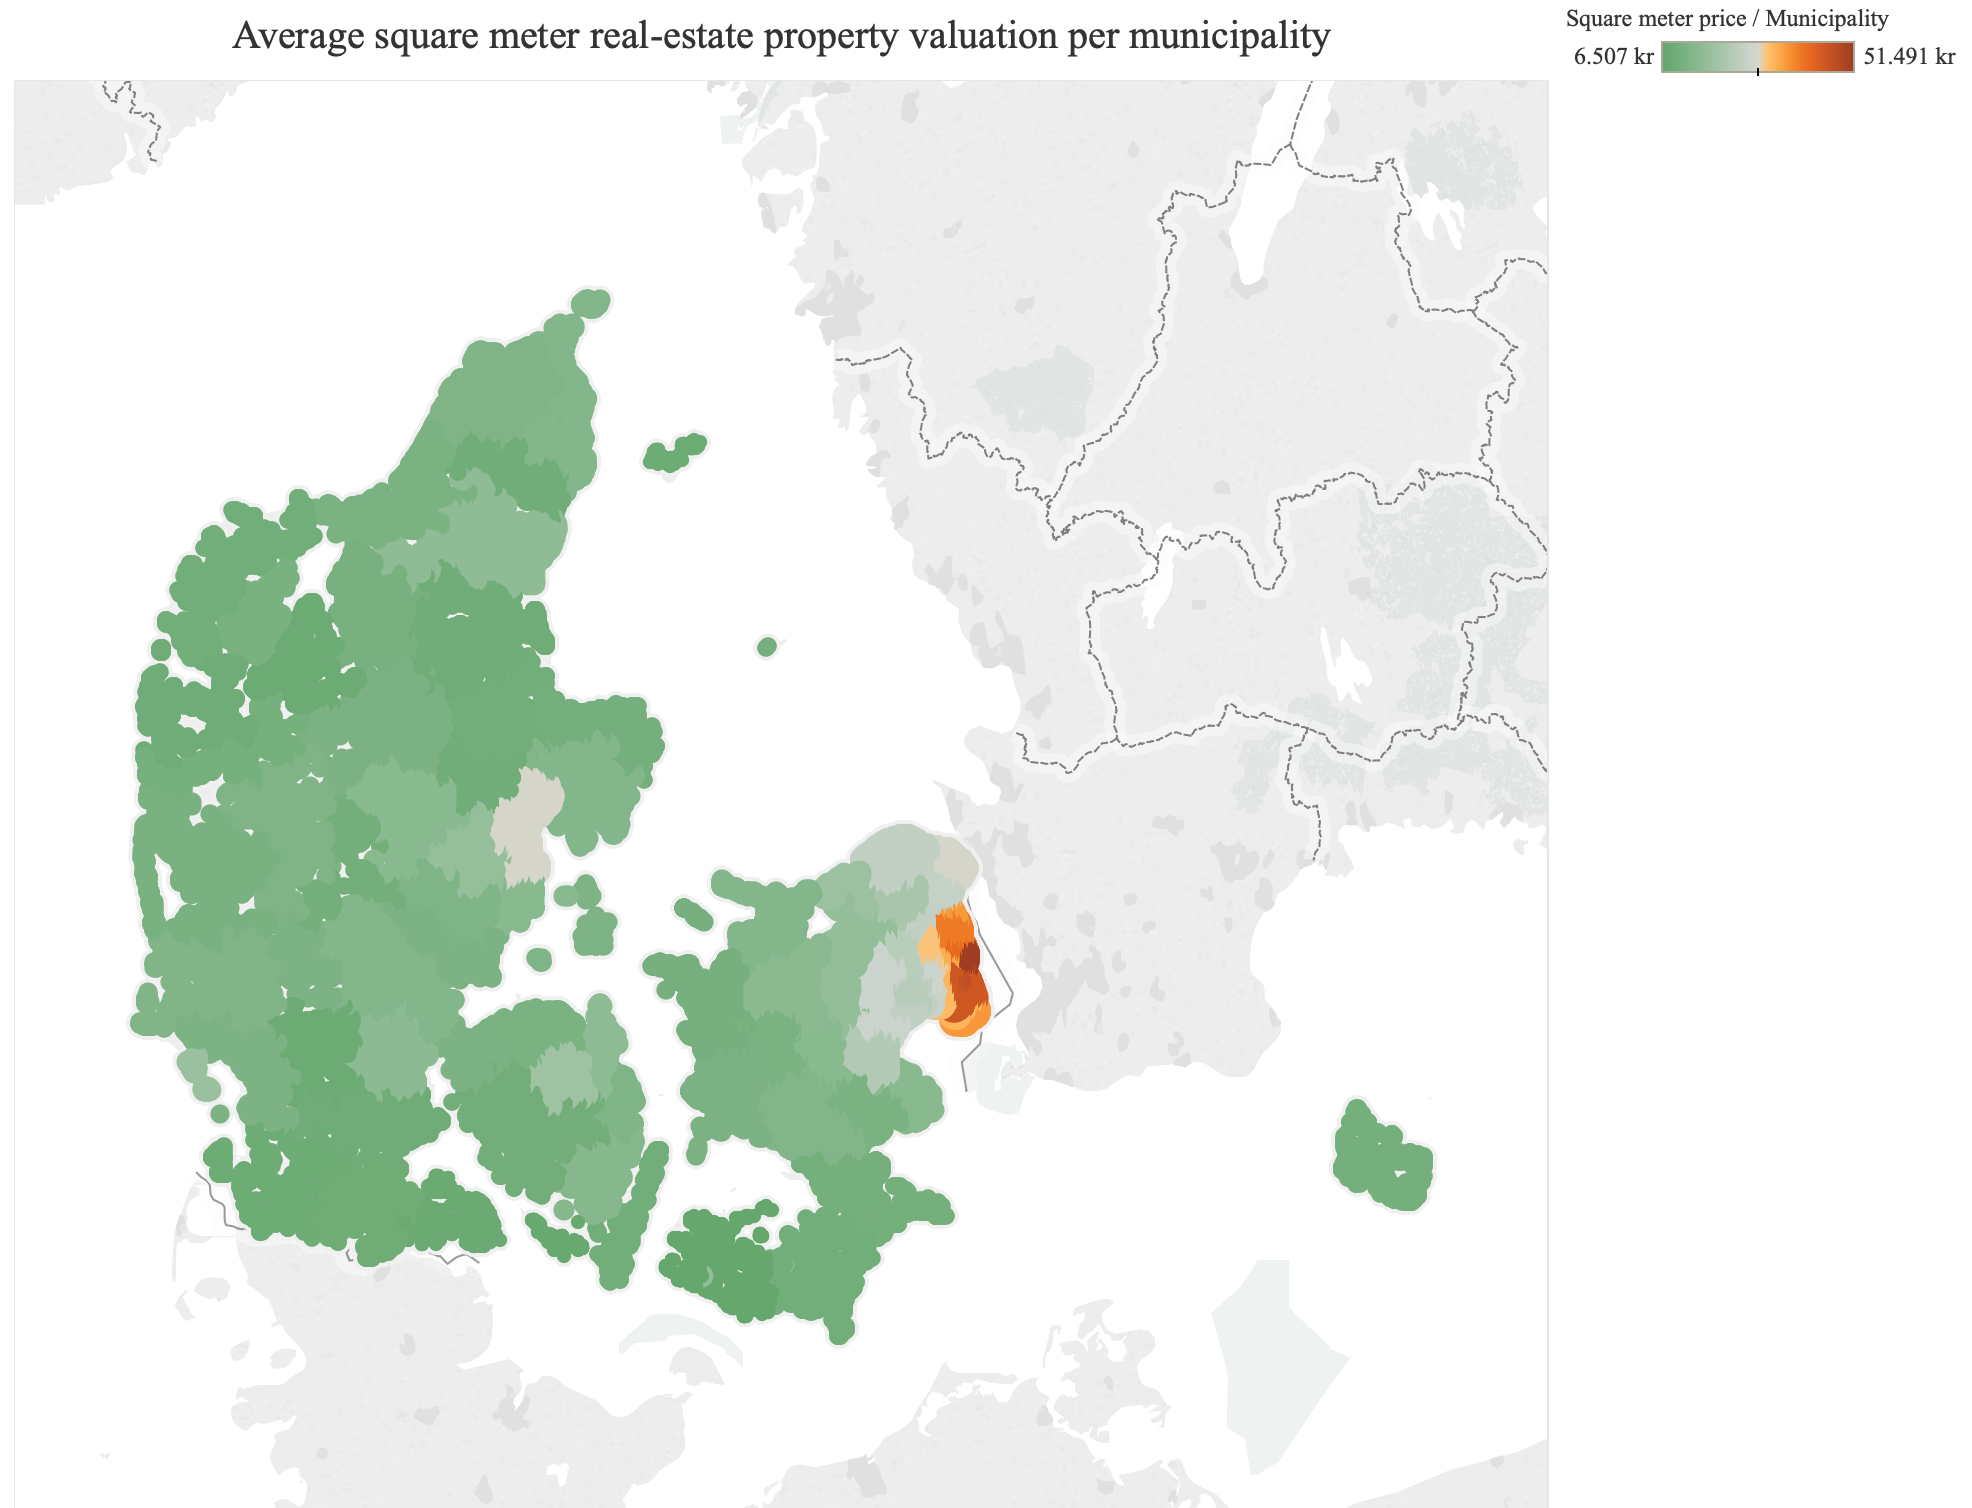
\includegraphics[scale=1]{123.png}
\end{figure}

Figure 1 shows the average square meter price valuation of active offers per municipality in Denmark. The maximum square meter price being approximately 8 times higher in the municipality of Gentofte, than Lolland, the municipality with lowest average square meter price valuations. A tendency visualized in the figure, is that average square meter price valuations are higher in in highly populated municipalities and in suburban areas surrounding Copenhagen. \newline

The valuations included in the research are collected from one of Denmarks largest online real-estate websites named Boliga.dk. The Boliga data contains approximately 66 thousand active offerings with valuations ranging from 15 thousand to 85 million. This research paper intends to analyze real estate price valuations and which effects geo- and sociodemographic criteria affect valuations, using machine learning models. Our research questions is as follows: 
Which features are most relevant for predicting evaluations of real estate properties in Denmark?

The research paper contains a section describing the construction of research data was performed explains the choices of gathering meaningful features for the machine learning model. Also, a section revolving the choice and optimization of machine learning models is included, where the intention is to provide insights on our progress on finding the optimal model. As a result, a preferable machine learning model is chosen with a discussion of its usability. 


\section{Literature Review}

\section{Data Description \& Ethics}

\subsection{Ethical Considerations in the Current Research Project}
In the current paper the appropriate care and consideration has been given to the ethical concerns regarding the scraping, processing, and the presentation of the data. Drawing upon the European Comissions\footnote{European Commission (2018). \textit{Ethics in Social Sciences and the Humanities}} ethical guidelines and principles for ethical conduct in social data science, the potential harm to users of Boliga's web-page were carefully considered. As a step to prevent the mosaic effect and in an effort to anonymize the scraped data only aggregated data will be presented in this paper, so that no single observation can be identified from the analysed data.\newline
No informed consent has been obtained from the users of the site, prompting us to consider the consequences of the lack thereof, as informed consent is paramount to the proper, ethical conduct in social science. However, sometimes, as in this instance, informed consent can be logistically impossible to collect from all participants in the study. Salganik mentions that informed consent for everything is an ideal, but in practice impossible to obtain and researchers should instead strive to follow an alternative rule, that he describes as: "some form of consent for most things." \footnote{Salganik, Matthew J. (2019) \textit{Bit by Bit Bit - Social research in the digital age.} p.281} Adhering to this, more complex  understanding of the practicality of informed consent, we chose to contact Boliga to inform them of our intent to scrape their website and use the data in an educational context. Boliga responded positively to our inquiry, which we took as informed consent from a third party on behalf of the participating users in our study.\newline
In considering the legal ramifications of our research and to make sure we adhere to the seven principles of GDPR, and other appropriate legislation and legal contracts, we consulted the general guidelines introduced by the Consumer Data Research Center. In particular we noted that we are justified to collect and use the data on the lawful basis of legitimate interests. Furthermore, we consulted with Boliga's Terms and Conditions to avoid any legal ramifications and the appropriate contractual terms of interest can be seen in \href{https://www.boliga.dk/vilkaar-og-betingelser}{§10 Terms and Conditions}. In order to comply with these terms we refrained from burdening their website's performance by implementing a time.sleep function, which causes each scraping iteration to pause for 0.5 seconds before commencing on scraping the next page (see appendix XX). Furthermore, Boliga prohibits the use of automated scrapers and bots, which we did not do, as our scraping was done in a specified time-frame and we did not automate the procedure to be done on multiple occasions.
\subsection{Data Scraping Process}
In the following paragraphs our scraping efforts will be described. The scrapers can be examined in the attached Jupyter Notebooks labelled \textcolor{red}{XX and XX.} 
\paragraph{\href{https://www.boliga.dk}{Boliga}\newline}
Our data comes from \href{https://www.boliga.dk}{Boliga.dk}, the largest independent online web-portal for real-estate sales in Denmark and has access to unique features such as "liggetid", price-development and access to BBR - the Danish Building and Housing Register \footnote{\href{https://www.boligagruppen.dk}{www.boligagruppen.dk}}. Giving us unique insights into the pricing of real-estate in all 98 municipalities of Denmark. At the time of scraping 65,950 properties were for sale.\newline
The scraping process was conducted on Friday the 23rd of August 2019. We had advised Boliga of our intent to collect data from their website via our scraper in an effort to identify ourselves and our intent\footnote{Shiab, Nael (2015) \textit{On the Ethics of Web Scraping and Data Journalism. Global Investigative Journalism Network.}}. In order to scrape the data of interest we familiarized ourselves with the HTML-structure of Boliga. On the basis of these insights we constructed a code, which were able to scrape every page, containing information pertaining the currently listed real-estates on Boliga. The scraper requested all information available from each individual page, which surmounted to 1,319 URL requests. \newline
For each URL, 34 features and the target variable (price) was collected. Table \textcolor{red}{XX} provides an overview of the features with a short description, and whether the feature has been dropped or saved for later usage. There are three reasons for a feature to be dropped:\newline
1. The feature does not act with independent characteristics according to the research,\newline
2. The feature contains insufficient data,\newline
3. The feature is poorly formatted and cannot efficiently be recreated. 
\vspace*{10px} \newline
\textit{Features Obtained:} \newline
\begin{tabular}{c c}
Continuous: & basementSize, buildYear, Ejerudgift, lotSize	, price, rooms, size  \\	
\end{tabular}\newline 
\begin{tabular}{c c}
Categorical: & ForClosure, Type, Municipality, lotSize	, price, rooms, size  \\	
\end{tabular}\newline 

\paragraph{\href{https://www.hvorlangterder.dk}{Hvorlangterder.dk}\newline}
\href{https://www.hvorlangterder.dk}{hvorlangterder.dk} returns distances from a given address, to conveniences such as supermarkets, hospitals and schools.   
The scraping of \href{https://www.hvorlangterder.dk}{hvorlangterder.dk} was achieved by writing a function that took in the GPS-coordinates gathered from Boliga and a list of points of interest. It constructed a URL (65,950 URL request), which was scraped and the json response was returned as a dictionary of distances to the points of interest. The values from each key in the dictionary was then extracted as a new column in a Pandas DataFrame.\newline
As Jupyter performs poorly at running long asynchronous tasks and estimated a running time of 18 hours this procedure was run in Visual Studio.
 \vspace*{10px} \newline
\textit{Features obtained:}\newline
\begin{tabular}{c c}
Distances to: & lake, forest, doctor, supermarket,	school, daycare, hospital, train \\	
\end{tabular}\newline 
\begin{tabular}{c c}
\qquad \qquad \qquad \qquad &  pharmacy, library, coast, junction \\	
\end{tabular}\newline 
\paragraph{Social and economic factors\newline}
Social and economic factors on municipality level is collected from \href{https://statistik.politi.dk/QvAJAXZfc/opendoc.htm?document=QlikApplication%2F2999_Public\%2FPublic_IndsatsResultater.qvw}{statistik.politi.dk} and  
\href{https://www.dst.dk/da/Statistik/emner/befolkning-og-valg}{Danmarks Statistik} respectively. These factors includes income, reported crime and level of highest completed education etc. These are transformed to into ratios, by taking the total population in a given municipality into account.   
 \vspace*{5px} \newline
\begin{tabular}{c c}
\textit{Features obtained:}: & Relativ Ledighed, Grundskole, Gymnasiale uddannelser \\	
\end{tabular}\newline 
\begin{tabular}{c c}
\qquad \qquad \qquad \qquad \quad & Erhvervsfaglige uddannelser,	 KVU, 	MVU, Bacheloruddannelser  \\	
\end{tabular}\newline 
\begin{tabular}{c c}
\qquad \qquad \qquad \qquad \quad & LVU, Kommunal\_gennemsnitsinkomst\_2017, Total\_reported\\	
\end{tabular}\newline 
\begin{tabular}{c c}
\qquad \qquad \qquad \qquad \quad & Population\_in\_urban\_development  , Socioeconomic\_index \\	
\end{tabular}\newline 
\begin{tabular}{c c}
\qquad \qquad \qquad \qquad \quad & average\_class\_size	expenses\_sport\_and\_other\_cultural\_activities	  \\	
\end{tabular}\newline 
\begin{tabular}{c c}
\qquad \qquad \qquad \qquad \quad & , expenses\_per\_school\_student	   \\	
\end{tabular}\newline 
% 				average_class_size	expenses_sport_and_other_cultural_activities
\subsection{Merging Data}

\subsection{Data Cleaning}

A few of the listed housing, have been listed for over a decade. These are considered outliers, which are overly priced considering their characteristics. The outliers are excluded, because they would otherwise only contribute to further bias of overestimation. The total number of excluded housing are approximately 4000.  

\subsection{Descriptive Statistics}
\begin{table}[h!]
\begin{center}
\caption{Key Statistics\label{time}}
\begin{tabular}{| c | c | c | c | c | c |} 
\hline
   & Price & \, Rooms \ & \ $m^2$ \ & Average Municipal Income \\ \hline
   Mean & 2,312,798.00 & \ 4.21 \  & \ 127.82 \ & 312,957.03 \\ \hline
   Std & 2,351,127.00 & 2.12 & 75.67 & 46,095.34 \\ \hline
   Min & 15,000.00 & 0 & 0 & 257,776 \\ \hline
   25\% & 985,000.00 & 3 & 82 & 290,973 \\ \hline
   50\% & 1,695,000.00 & 4 & 123 & 302,153 \\ \hline
   75\% & 2,895,000.00 & 5 & 167 & 318,745 \\ \hline
   Max & 85,000,000.00 & 50 & 2,390 & 583,331 \\ \hline
\end{tabular}
\end{center}
\end{table} 
\begin{figure}[H]
  \centering
   \caption{}
   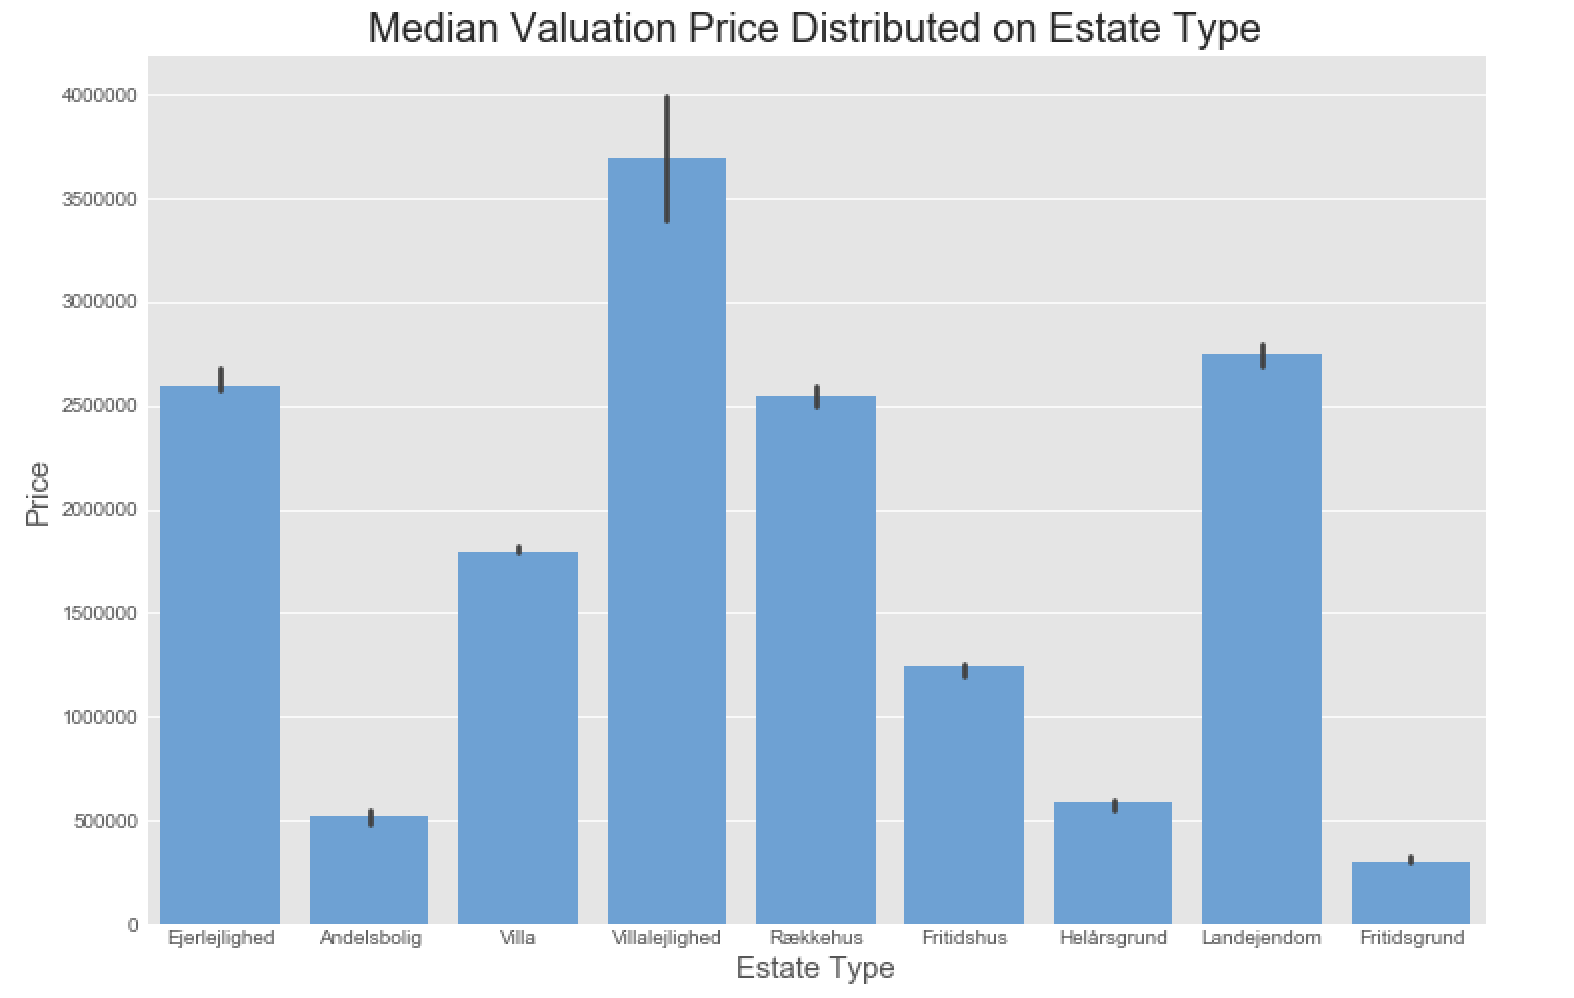
\includegraphics[width=\linewidth]{Barplot_Estate2.png} 
  \label{fig:}
\end{figure}




\subsubsection{The Dataset}
The merged dataset contains 61.618 observations and 37 features.   The features are of both categorical and continuous measures. \newline 



\subsubsection{Selecting Features}


\section{Methods}
\subsection{Supervised Machine Learning}
The objective by applying Machine Learning is to train a model that can predict pricing of housing listed in near future.
Two types of predictive models will be used for the sake of returning different outputs: Regression-model to return the pricing as a continuous output. As well as a classification-model for predicting the interval which the price is included in. 
\subsection{Fitting the model}
The potential problems of underfitting and overfitting should be assessed when fitting a model. A model is underfitted if it hardly captures the variation of the sample data. It is then said that the model has \textit{high bias}. A model is overfitted, when it is overly sensitive to the idiosyncrasy of the sample data and captures the variation in too great detail. This problem often comes with the introduction of a sizeable number of features. Overfit models are said to have \textit{high variance}\footnote{Rashka, Sebastian; Mirjalli, Vahid; \textit{Python Machine Learning, Machine Learning and Deep Learning with Python, scikit-learn, and Tensorflow}. p.73}. In both cases, the model will generalize poorly. A key step in defining a decent model in machine learning is to find an optimal bias-variance-balance, by tuning the complexity of one’s model. This is done through \textit{regularization}. In this project three different types of regularization are applied; Lasso, Ridge and Elastic net.   

\subsubsection{Lasso}
Regularization by Lasso, will penalize complexity of the model by the sum of the absolute value of the coefficients. This penalty will make the model less complex and more appropriate for prediction.  \footnote{Foster, Ian; Rayid Ghani Ron S. Jarmin, Frauke Kreuter, Julia Lane; \textit{Big Data in Social Sciences, A Practical Guide to Methods and Tools} p. 173}\, \footnote{Rashka, Sebastian; Mirjalli, Vahid; \textit{Python Machine Learning, Machine Learning and Deep Learning with Python, scikit-learn, and Tensorflow} p. 332}
\newline Lasso minimizes: $$L_{Lasso}(\hat{\beta}) = \left(\sum_{i=1}^{n} (y_i-\hat{y_i}(\beta))^2+\lambda\sum_{j=1}^{p}|\hat{\beta_j}|\right) \qquad s.t \quad \lambda \geq 0 $$
Another convenient attribute of the Lasso penalty is that some estimates are set equal to zero and thereby produce sparse models\footnote{Hal R. Varian. \textit{Big data: New tricks for econometrics. Journal of Economic Perspectives}. p.19}. Lasso thereby performs the feature selection automatic.   
\subsubsection{Ridge}
The ridge model penalizes with the sum of squared coefficients. Opposed to Lasso, Ridge do not force features to be omitted. Ridge minimizes:
$$L_{Ridge}(\hat{\beta}) = \left(\sum_{i=1}^{n} (y_i-\hat{y_i}(\beta))^2+\lambda\sum_{j=1}^{p}\hat{\beta_j}^2\right) \qquad s.t \quad \lambda \geq 0 $$ 
The Ridge model add bias in exchange for a decrease in variance, resulting in a better prediction model. 

\subsubsection{Elastic-net}
The Elastic net is a combination of Lasso and Ridge. Elastic net minimizes the function: 
$$L_{elasticnet}(\hat{\beta}) = \frac{\sum_{i=1}^{n}\left(y_i-\hat{y_i}(\beta)\right)^2}{2n} + \lambda\left(\frac{1-\alpha}{2}\sum_{j=1}^{p}\hat{\beta_j}^2+\alpha\sum_{j=1}^{p}|\hat{\beta_j}|\right)$$
$$0 \leq \alpha \leq 1 \quad \wedge \quad \lambda \geq 0$$
Where $\alpha$ denotes the relative mixing between Lasso and Ridge. 
\subsection{Optimizing the Hyperparameter}
To minimize the mean squared errors of our Lasso and Ridge regression we performed k-fold cross validation to optimize the hyperparameter $\lambda$. 
We split the data into a test set and a development set, consisting of respectively 20\% and 80\% of the total observations. Subsequently, we use k-fold cross-validation to randomly split the development set into k folds, where k-1 folds are used to train the model. The remaining fold is used to validate the model’s generalizability by calculating the mean squared errors of the trained model’s prediction of the left-out fold\footnote{Rashka, Sebastian; Mirjalli, Vahid; \textit{Python Machine Learning, Machine Learning and Deep Learning with Python, scikit-learn, and Tensorflow}. p.191}. This process is repeated k times and each time a new fold is left out for validation. Since we are working with a relatively large dataset we chose to split our data into 5 folds, and computed the average MSE for the 5 iterations. By using the k-fold cross-validation method we relieve ourselves of the concern that the estimation of our model’s performance is simply due to a lucky or unlucky split of the data. \newline
We performed this procedure for 12 different values of $\lambda$ spanning between \textcolor{red}{$10^(-4) and 10^4$}. We chose the value of $\lambda$ which yields the smallest average MSE over the 5 folds. 
We both calculated the optimal hyperparameters for a Ridge regression model, a Lasso regression model and an Elastic Net regression model. \textcolor{red}{The following table} shows the performance of the different models, when trained with their optimal hyperparameter and predicting the test data.
\section{Analysis}

\begin{table}[h!]
\begin{center}
\caption{Key Statistics\label{time}}
\begin{tabular}{| c | c | c | c | c | c |} 
\hline
   & Price & \, Rooms \ & \ $m^2$ \ & Average Municipal Income \\ \hline
   Mean & 2,312,798.00 & \ 4.21 \  & \ 127.82 \ & 312,957.03 \\ \hline
   Std & 2,351,127.00 & 2.12 & 75.67 & 46,095.34 \\ \hline
   Min & 15,000.00 & 0 & 0 & 257,776 \\ \hline
   25\% & 985,000.00 & 3 & 82 & 290,973 \\ \hline
   50\% & 1,695,000.00 & 4 & 123 & 302,153 \\ \hline
   75\% & 2,895,000.00 & 5 & 167 & 318,745 \\ \hline
   Max & 85,000,000.00 & 50 & 2,390 & 583,331 \\ \hline
\end{tabular}
\end{center}
\end{table}

\section{Results}

\section{Discussion}
\subsection{Data critique}
Another interesting prediction which could have been obtained using the same methods, would have been to estimate expected selling prices. This could have been done simply by scraping data on sold housing instead. This could be of more value for private agents, whose main interest should be the selling price of their housing. 
\newline 
In a prediction-model like this it is near impossible to evade some form of omitted variable bias. A significant amount of potential important factors can not be acquired. For an example the view from the listed housing will for sure have great impact of the valuation price. Another factor of interest could have been a evaluation of the condition of the housing, unfortunately the "statement of property" red. (tilstandrapport) are not publicly accessible. \newline
The prediction of the cooperative housing valuation %\footnote{http://housingpeople.dk/en/housing-guide/housing-types/cooperative-andelsbolig/},
are subject to significant bias, since the cooperative housing that enters the marked through a realtor often would be those with critical amount of undesirable characteristics. 


\section{Conclusion}

\section{An Ethical Overview}

The ethical principles of social research are anchored in the fundamental human rights, which are broadly formulated in the UN Declaration of Human Rights. Additional policies and declarations that codify principles of research ethics and the ethical treatment of research participants include the Nuremberg Code, the Helsinki Declaration, the Belmont Report, and the Menlo Report\footnote{Salganik, Matthew J. (2019) \textit{Bit by Bit Bit - Social research in the digital age.}}\, \footnote{European Commission (2018). \textit{Ethics in Social Sciences and the Humanities}}. These codes and addendums originate mostly in the biomedical field, though they encompass the central principles applied to all human research, which have led some academics to call for a Hippocratic oath for data scientists to safeguard against powerful new technologies under development in laboratories and tech firms\footnote{Rotblat, Joseph (1999) \textit{A Hippocratic Oath for Scientists}}\, \footnote{Sample, Ian (2019, Fri 16 Aug 2019) \textit{and tech specialists need Hippocratic oath, says academic.}}. This discussion is nothing new however, as a tentative reformulation of the Hippocratic oath was introduced by Karl Popper\footnote{Popper, Karl (1969) \textit{The Moral Responsibility of the Scientist}}, wherein he stressed the importance of professional responsibility, a critical mind, and an overriding loyalty towards the betterment of mankind.\newline
Matthew Salganik offer four principles deduced from the Belmont and Menlo Report that should guide the ethical deliberations of the researcher: 1) the respect for persons, that is individuals should be treated as autonomous and if circumstances require it individuals should be entitled to additional protections. 2) Beneficence stresses the importance of doing no harm and to maximize the possible benefits and minimizing any potential harms. 3) The principle of justice touches upon the importance of the distribution of burdens and benefits of the social scientist's research. This principle stress that is should not be a single stratum of society that bears the costs of the research while another stratum benefits. 4) The fourth and final principle is the respect for law and public interest, according to Salganik, the principle consists of two distinct elements, that is compliance to relevant laws and legal contracts and transparency-based accountability. It is worth noting that Popper’s tentative Hippocratic oath mirrors the first three principles put forth by Salganik, stressing the importance of the ethical conduct of the researcher.\newline
The need for rigid ethical standards within computational social science was made apparent by the Cambridge Analytica Scandal that broke on the 17th of March 2018. Where Steve Bannon could reveal that between 2013 and 2015 Cambridge Analytica had exploited a loophole in Facebook’s API which allowed the company to harvest profile data from 87 million Facebook users, without the user’s permission and use the harvested data to construct a massive targeted marketing database based on the user’s likes and interests\footnote{Vox.com (2018) \textit{The Cambridge Analytica Facebook scandal} [Online]}. Other examples of misuse of data acquired from Facebook include the Harvard-run experiment, where students' data was used to create new knowledge about how social networks form and how these networks and their actors' behavior co-evolve, and the emotional contagion experiment from 2012, where approximately 700,000 users were involved in a research experiment to examine the extent to which a person's emotions are affected by the emotions of the people they interact with (Salganik. 2019).\newline
From this it should be evident that clear ethical guidelines are required in order to protect the user's privacy from tech-savvy companies. To this end, the European Parliament introduced the General Data Protection Regulation (GDPR). With its seven overarching principles the GDPR seeks to formalize the procedures involved in the data processing and storing of sensitive and private information (CDRC\footnote{Consumer Data Research Center, UK  [CDRC] (2018) \textit{The General Data Protection Regulation \& Social Science Research} [Online]:}). These principles include and expand upon the principles found in the Belmont and Menlo Report. The most important consideration, however, must be that even a dataset comprising tens of thousands of observations involve human beings who must be protected from adverse side-effects of the social research. There is considerable evidence that point to the fact that even in anonymized data sets it can be possible to backtrack an individual's identity. A researcher must therefore be mindful of the mosaic effect if the dataset combines large amount of data from various sources (European Commission 2018).

\newpage
\section{Litterature}
\ Foster, Ian; Rayid Ghani Ron S. Jarmin, Frauke Kreuter, Julia Lane; \textit{Big Data in Social Sciences, A Practical Guide to Methods and Tools}, CRS Press 2017

Rashka, Sebastian; Mirjalli, Vahid; \textit{Python Machine Learning, Machine Learning and Deep Learning with Python, scikit-learn, and Tensorflow}, $2^{nd}$editon, Packt Publishing 2017.

Hal R. Varian. \textit{Big data: New tricks for econometrics. Journal of Economic Perspectives}, 28(2):3–28, 2014. 

Consumer Data Research Center, UK  [CDRC] (2018) \textit{The General Data Protection Regulation \& Social Science Research} [Online]: \href{https://ec.europa.eu/research/participants/data/ref/h2020/other/hi/h2020_ethics-soc-science-humanities_en.pdf}{ec.europa.eu/research/participants/data/ref/h2020/other/hi/h2020\_ethics-soc-science-humanities\_en.pdf} [Accessed on 25/08/2019]

European Commission (2018). \textit{Ethics in Social Sciences and the Humanities} [Online]: \href{https://ec.europa.eu/research/participants/data/ref/h2020/other/hi/h2020_ethics-soc-science-humanities_en.pdf}{https://ec.europa.eu/research/participants/data/ref/h2020/other/hi/h2020\_ethics-soc-science-humanities\_en.pdf} [Accessed on 25/08/2019] 

Popper, Karl (1969) \textit{The Moral Responsibility of the Scientist}. Encounter, March 1969, pp. 52-56 [Online]: \href{http://www.unz.com/print/Encounter-1969mar-00052}{http://www.unz.com/print/Encounter-1969mar-00052} [Accessed on 25/08/2019]

Rotblat, Joseph (1999) \textit{A Hippocratic Oath for Scientists}. Science, November 1999: Vol. 286, Issue 5444, pp. 1475 [Online]: \href{https://science.sciencemag.org/content/286/5444/1475.full}{https://science.sciencemag.org/content/286/5444/1475.full} [Accessed on 25/08/2019] DOI: 10.1126/science.286.5444.1475 

Salganik, Matthew J. (2019) \textit{Bit by Bit Bit - Social research in the digital age.} Princeton, NJ: Princeton University Press.

Sample, Ian (2019, Fri 16 Aug 2019) \textit{and tech specialists need Hippocratic oath, says academic.} The Guardian [Online]: \href{https://www.theguardian.com/science/2019/aug/16/mathematicians-need-doctor-style-hippocratic-oath-says-academic-hannah-fry} [Accessed on 25/08/2019]

Vox.com (2018) \textit{The Cambridge Analytica Facebook scandal} [Online]: \href{https://www.vox.com/2018/4/10/17207394/cambridge-analytica-facebook-zuckerberg-trump-privacy-scandal} [Accessed on 26/08/2019] 

Boligagruppen.dk (2019) \textit{Om boliga gruppen} [Online]: \href{https://www.boligagruppen.dk}{www.boligagruppen.dk}: [Accessed on 27/08/2019]

Shiab, Nael (2015) \textit{On the Ethics of Web Scraping and Data Journalism. Global Investigative Journalism Network.} [Online]: \href{https://gijn.org/2015/08/12/on-the-ethics-of-web-scraping-and-data-journalism/}{gijn.org/2015/08/12/on-the-ethics-of-web-scraping-and-data-journalism/}: [Accessed on 27/08/2019]
\end{document}